\documentclass[conference]{IEEEtran}
\IEEEoverridecommandlockouts
% The preceding line is only needed to identify funding in the first footnote. If that is unneeded, please comment it out.
\usepackage{cite}
\usepackage{amsmath,amssymb,amsfonts}
\usepackage{algorithmic}
\usepackage{graphicx}
\usepackage{textcomp}
\usepackage{amssymb}
\usepackage{float} % for H placement option
\usepackage{listings}
\usepackage{xcolor}
\def\BibTeX{{\rm B\kern-.05em{\sc i\kern-.025em b}\kern-.08em
    T\kern-.1667em\lower.7ex\hbox{E}\kern-.125emX}}
\begin{document}

\title{Hard disk failure data analysis\\}

\author{\IEEEauthorblockN{Luca Falasca}
\IEEEauthorblockA{\textit{0334722} \\
luca.falasca@students.uniroma2.eu
}
\and
\IEEEauthorblockN{Matteo Conti}
\IEEEauthorblockA{\textit{0323728} \\
matteo.conti97@students.uniroma2.eu
}\\
}


\maketitle
\thispagestyle{plain}
\pagestyle{plain}

\begin{abstract}
\end{abstract}

\section{Introduzione}
\subsection{Descrizione del problema}
Il problema da affrontare consiste nell'eseguire il batch processing di dati di grandi dimensioni mediante l'uso di una pipeline basata su framework per Big Data. Nello specifico, l'obiettivo è analizzare un dataset contenente informazioni relative ai fallimenti dei dischi rigidi attraverso l'esecuzione di 3 query.

\subsection{Obiettivi}
Gli obiettivi del progetto sono quelli di eseguire le query proposte e di valutare le prestazioni di esse a partire da due formati di file, CSV e Parquet. Il motivo della scelta di Parquet è perché essendo un formato basato su colonne, risulta essere più efficiente per le query di aggregazione e quindi in fase di progettazione analizzando le query ci è sembrato più adeguato utilizzarlo rispetto ad altri formati per righe.

\subsection{Dataset}
Il dataset fornito è una versione ridotta di quello presentato nel Grand Challenge della conferenza ACM DEBS 2024. Delle numerose colonne presenti nel dataset, ne verranno selezionate solamente cinque per l'esecuzione delle query, in particolare:
\begin{itemize}
    \item \textit{date}: data della misurazione
    \item \textit{serial\_number}: identificativo del disco rigido
    \item \textit{failure}: indica se il disco rigido ha avuto una failure o meno
    \item \textit{model}: modello del disco rigido
    \item \textit{vault\_id}: identificativo del gruppo di storage server
    \item \textit{s9\_power\_on\_hours}: ore di accensione del disco rigido
\end{itemize}
Esplorando il dataset si può notare una ambiguità nella colonna \textit{s9\_power\_on\_hours}, essa contiene dei valori 0. Questi valori possono essere interpretati in due modi:
\begin{itemize}
    \item Il dato è errore di misurazione e quindi va eliminato
    \item Il disco rigido è stato acceso per meno di un'ora al momento della misurazione
\end{itemize}
Date le seguenti considerazione si è deciso di non eliminare i valori 0 e considerarli quindi validi. Questo andrà ad influenzare i risultati della query 3, in particolare sarà particolarmente evidente per quanto riguarda il minimo delle ore di accensione.
La colonna \textit{s9\_power\_on\_hours} contiene anche diversi valori nulli, le righe corrispondenti verranno eliminate in fase di preprocessamento.
Inoltre la colonna \textit{vault\_id} contiene elementi il cui valore non è un intero bensì la stringa "vault\_id", anche questa volta le righe corrispondenti verranno eliminate in fase di preprocessamento.

\section{Pipeline}
Per la gestione dei dati relativi ai guasti dei dischi rigidi, è stata implementata una pipeline containerizzata il cui deploy è stato fatto tramite docker compose. La pipeline è composta da diverse componenti, ognuna delle quali svolge un compito specifico, in particolare sono stati utilizzati Apache NiFi per la data ingestion, HDFS per il data storage, Spark per il data processing e MongoDB per l'analytical data storage, di seguito verrano illustrati i dettagli di ciascuna componente.
\begin{figure}[H]
    \centering
    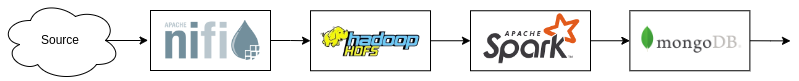
\includegraphics[width=0.5\textwidth]{./res/pipeline_2.png}
    \caption{Pipeline ad alto livello}
    \label{fig:pipeline}
\end{figure} 
\subsection{Data Ingestion}
Per la data ingestion è stato utilizzato il framework Apache NiFi, il quale permette di creare dei flussi di dati a partire da diversi tipi di sorgente, definire delle operazioni di trasformazione su di essi e andare a memorizzare il risultato delle trasformazioni in sink di vario genere. Nel nostro caso NiFi svolge le seguenti operazioni:
\begin{enumerate}
    \item Riceve, tramite HTTP, il file CSV contenente i dati relativi ai guasti dei dischi rigidi
    \item Esegue una query SQL %(Fig. \ref{fig:nifi_query}) 
    per selezionare solamente le cinque colonne di interesse del CSV ed effettuare una pulizia dei dati rimuovendo righe contenenti valori nulli o invalidi. 
    \item Effettua l'assegnazione esplicita dello schema ai dati, se questo non viene fatto NiFi non riconosce correttamente il tipo di alcune colonne del dataset, interpretandole come delle strutture
    \item Scrive i dati su HDFS in formato Parquet e CSV
\end{enumerate}

Per implementare il flusso NiFi sono stati utilizzati diversi processors e controller services, in particolare:
\begin{itemize}
    \item \textit{ListenHTTP}: per ricevere il file CSV tramite HTTP
    \item \textit{QueryRecord}: per eseguire la query SQL ed effettuare l'assegnazione dello schema
    \item \textit{CSVReader}: per specificare a QueryRecord come è fatto il flusso che riceve in input
    \item \textit{CSVSetWriter}: per specificare a QueryRecord come deve essere il flusso che genera in output
    \item \textit{AvroSchemaRegistry}: per specificare a CSVReader e CSVSetWriter lo schema dei dati
    \item \textit{PutHDFS}: per scrivere i dati su HDFS
    \item \textit{PutParquet}: per scrivere i dati su HDFS in formato Parquet
    \item \textit{UpdateAttribute}: per specificare che nome dare al flusso e di conseguenza il nome del file che verrà salvato su HDFS
\end{itemize}
% \begin{figure}[H]
%     \centering
%     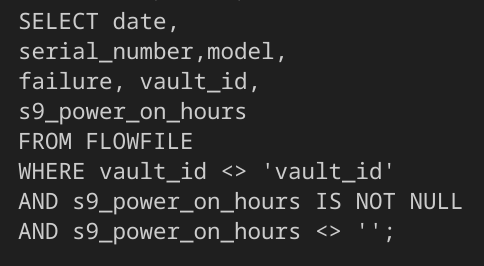
\includegraphics[width=0.4\textwidth]{./res/query_nifi.png}
%     \caption{Query SQL filtraggio dati NiFi}
%     \label{fig:nifi_query}
% \end{figure} 
\begin{figure}[H]
    \centering
    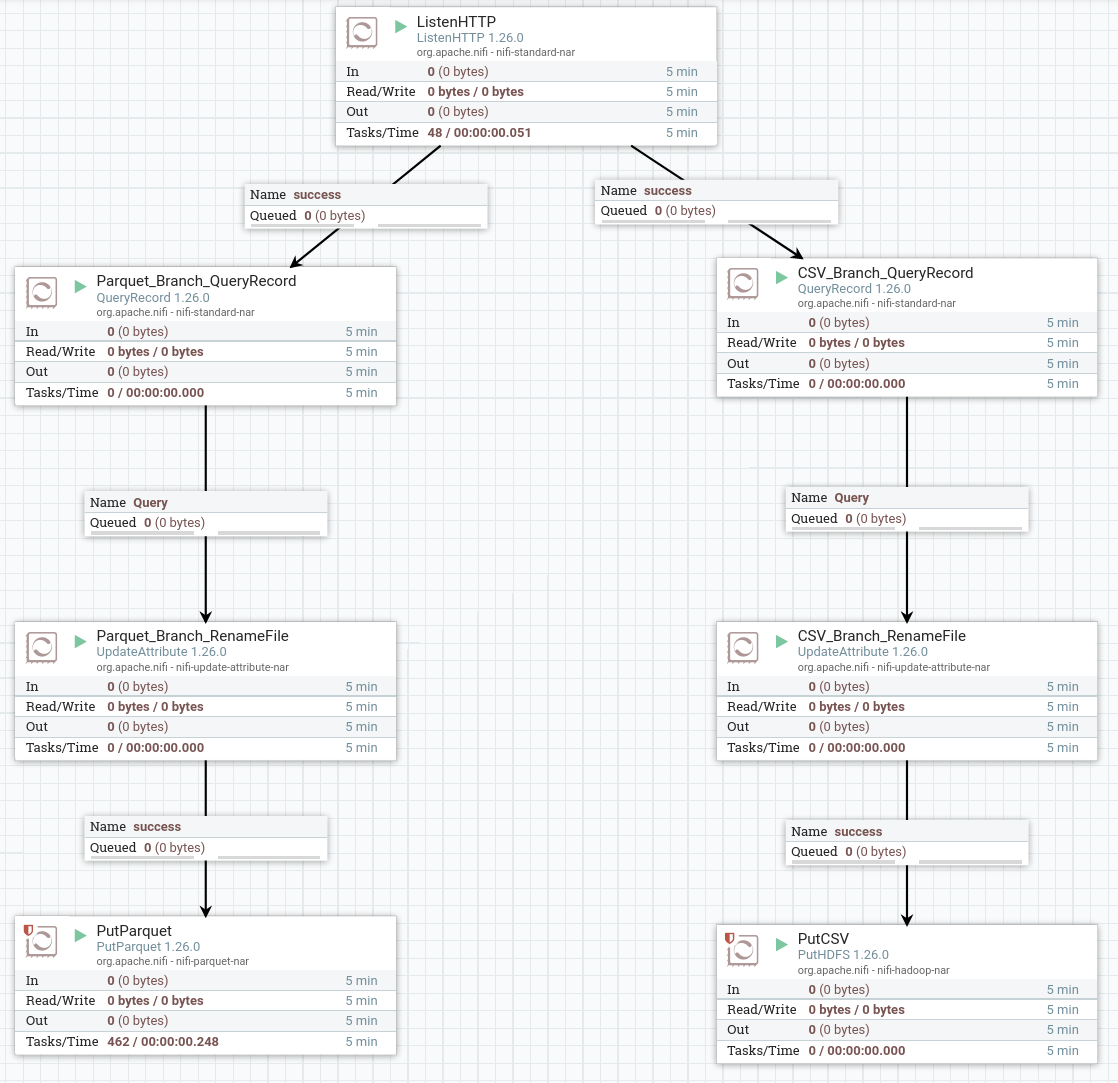
\includegraphics[width=0.4\textwidth]{./res/nifi_flow.png}
    \caption{Nifi flow}
    \label{fig:nifi_flow}
\end{figure} 
\subsection{Data Storage}
Come data lake in cui memorizzare i dati a a seguito del preprocessamento effettuato da parte di NiFi è stato utilizzato HDFS, il quale permette di memorizzare grandi quantità di dati su un cluster di nodi. Nel nostro caso il cluster è composto da:
\begin{itemize}
    \item 1 Namenode
    \item 2 Datanode
\end{itemize}
Non è stata utilizzata una struttura particolare per l'organizzazione dei file all'interno di HDFS, i file sono stati memorizzati tutti nella root directory.
\subsection{Data Processing}
Per il processamento dei dati e quindi l'esecuzione delle query è stato utilizzato il framework Spark, in particolare utilizzando la versione per python PySpark.Per queste query è stato utilizzato un cluster composto da uno spark master e quattro spark worker. Per farlo abbiamo utilizzato l'immagine bitami/spark nella versione 3.5.1. Per l'orchestrazione del cluster abbiamo utilizzato docker compose.
Il dataset filtrato è stato caricato dall'HDFS e i risultati delle query sono stati salvati in MongoDB utilizzando il connettore spark-mongodb.
Le query sono state eseguite sia a partire dal file in formato CSV che dal file in formato Parquet per valutare le differenze prestazionali tra un formato basato su colonne e uno basato su righe.
Per effettuare le query sono state utilizzate le API per i Dataframe e non quelli per gli RDD. 
Inoltre dato che le query sono formate principalmente da trasformazioni, l'azione che scatenerebbe la lazy evaluation, e quindi l'effettiva esecuzione della query, sarebbe la scrittura del risultato su MongoDB. Tuttavia, la durata della scrittura dipende dalla grandezza del risultato della query, il quale è abbastanza eterogeneo, abbiamo quindi deciso di unificare la metodologia di acquisizione delle misure di prestazioni inserendo un'azione di show() prima della scrittura su MongoDB.
\subsubsection{Query 1}
La query 1 prevede di calcolare per ogni giorno, per ogni vault (facendo riferimento al campo vault id), il numero totale di fallimenti, in particolare occorre determinare la lista di vault che hanno subito esattamente 4, 3 e 2 fallimenti.

Per prima cosa è stato fatto il drop delle colonne inutili per la query, che in questo caso sono \textit{serial\_number}, \textit{model} e \textit{s9\_power\_on\_hours}, successivamente è stato fatto il group by per \textit{date} e \textit{vault\_id} e la somma dei fallimenti (essendo i fallimenti rappresentati dai valori 0 e 1 la loro somma rappresenta il numero di fallimenti). Infine è stato effettuato un filtraggio che seleziona solo i vault che hanno subito un numero di fallimenti $\geq2$ e $\leq4$
\begin{figure}[H]
    \centerline{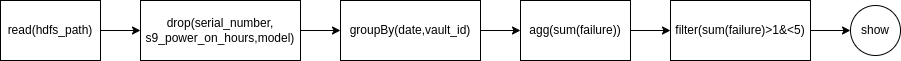
\includegraphics[width=0.5\textwidth]{res/query1_dag.png}}
    \caption{DAG di alto livello della query 1}
    \label{fig:dag_query1}
\end{figure}

\subsubsection{Query 2}
La query 2 è composta di due parti:
\begin{enumerate}
    \item Calcolare la classifica dei 10 modelli di hard disk che hanno subito il maggior numero di fallimenti, riportando il modello di hard disk e il numero totale di fallimenti subiti dagli hard disk di quello specifico modello
    \item Calcolare la classifica dei 10 vault che hanno registrato il maggior numero di
    fallimenti riportando, per ogni vault, il numero di fallimenti e la lista (senza ripetizioni) dei modelli di
    hark disk soggetti ad almeno un fallimento
\end{enumerate}
Anche in questo caso la prima cosa che viene fatta è il drop delle colonne inutili per la query, che in questo caso sono \textit{serial\_number}, \textit{s9\_power\_on\_hours} e \textit{date}, successivamente viene fatto un cache() per mantenere in memoria il Dataframe ed evitare di doverlo costruire più volte, in quanto esso verrà utilizzato per entrambe le parti della query.
Per la prima parte della query è stato fatto un group by per \textit{model} aggregando sulla somma di \textit{failure}, successivamente è stato fatto un ordinamento in ordine decrescente ed infine sono stati selezionati i primi 10 elementi.
Per la seconda parte della query vengono generati due dataframe, il primo facendo una group by su \textit{vault\_id} aggregando sulla somma di \textit{failure} ed il secondo filtrando i fallimenti $\geq1$ facendo una group by su \textit{vault\_id} e aggregando i \textit{model} in un set tramite collect\_set(). Successivamente i due dataframe vengono uniti tramite una join e sul campo \textit{vault\_id}, il dataframe ottenuto viene ordinato in modo decrescente sul campo \textit{failure}, infine vengono selezionati i primi 10 elementi.
\begin{figure}[H]
    \centerline{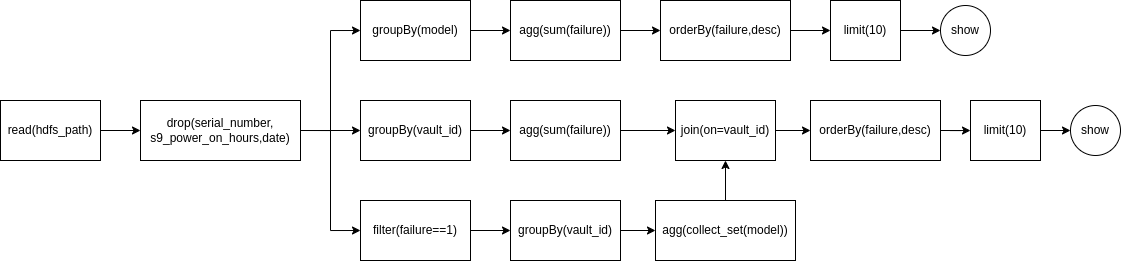
\includegraphics[width=0.5\textwidth]{res/query2_dag.png}}
    \caption{DAG di alto livello della query 2}
    \label{fig:dag_query2}
\end{figure}
\subsubsection{Query 3}
La query 3 prevede di calcolare il minimo, 25-esimo, 50-esimo, 75-esimo percentile e massimo delle ore di funzionamento (campo \textit{s9\_power\_on\_hours}) degli hark disk che hanno subito fallimenti e degli hard disk che non hanno subito fallimenti, indicando anche il numero totale di eveneti utilizzati per il calcolo delle statistiche.
Dato che il campo \textit{s9\_power\_on\_hours} è un campo cumulativo, per ottenere il tempo di funzionamento è necessario guardare la data più recente disponibile.
Anche in questo caso per prima cosa è stato fatto il drop delle colonne non necessarie che in questo caso sono \textit{model} e \textit{vault\_id}, successivamente è stato fatto un cache() per mantenere in memoria il Dataframe ed evitare di doverlo costruire più volte, in quanto esso verrà utilizzato per due operazioni diverse. A questo punto dal dataframe originale ne vengono generati altri due, uno che contenenete solamente dischi che hanno subito fallimenti ed uno che contenente solamente dischi che non hanno subito fallimenti. Per entrambi i Dataframe sono viene fatto un group by per \textit{serial\_number} e viene prelevato il valore più recente di \textit{s9\_power\_on\_hours} applicando alla colonna \textit{date} la funzione first(), la quale ne preleva la prima riga; questo è stato possibile in quanto il dataset è ordinato per data evitando di dover usare la funzione max() che avrebbe avuto un impatto maggiore sulle performance. Prima di eseguire il calcolo dei quantili è stato effettuato il drop delle colonne \textit{serial\_number} e \textit{date} in modo da tenere solamente il dato relativo delle ore di funzionamento per le failure 0 e 1 ed allegerire quindi le successive elaborazioni. Infine per il calcolo effettivo dei quantili è stata utilizzata la funzione approxQuantile() che permette di calcolare i quantili approssimati in modo efficiente, tramite essa è stato possibile calcolare anche il minimo ed il massimo che corrispondono rispettivamente al quanitle 0 e 100. Per generare il risultato della query è stato creato un nuovo dataframe contenente l'output di approxQuantile() e la count() delle righe utilizzate per il calcolo dei quantili per entrambi i dataframe (con e senza fallimenti).
\begin{figure}[H]
    \centerline{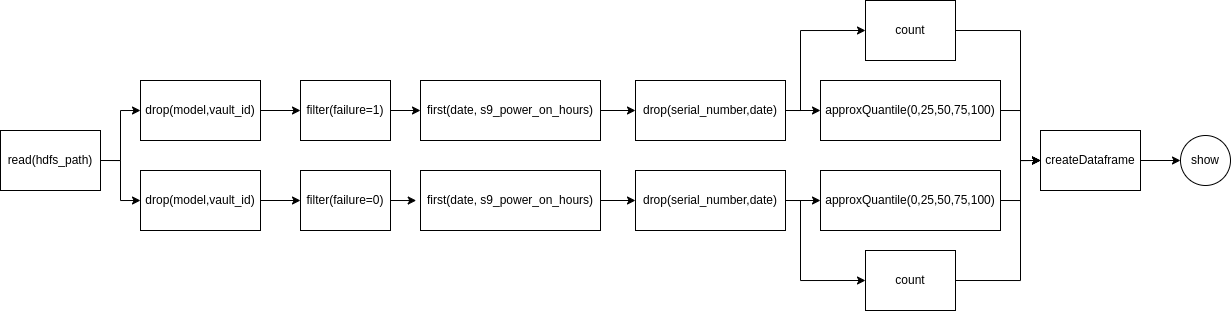
\includegraphics[width=0.5\textwidth]{res/query3_dag.png}}
    \caption{DAG di alto livello della query 3}
    \label{fig:dag_query3}
\end{figure}
\subsection{Analytical Data Storage}
I risultati delle query sono stati memorizzati in un database a documento, in particolare MongoDB (Fig. \ref{fig:mongo}).
Per organizzare i dati, è stata creata una collezione per ciascuna query, in cui ogni documento rappresenta una riga dei risultati ottenuti dalla query stessa. Inoltre, è stata creata un'altra collezione che contiene le performance, in particolare vengono riportati il timestamp dell'esperimento, la query, il formato del dataset su cui la query è stata eseguita ed il tempo di esecuzione della query stessa.
\begin{figure}[H]
    \centerline{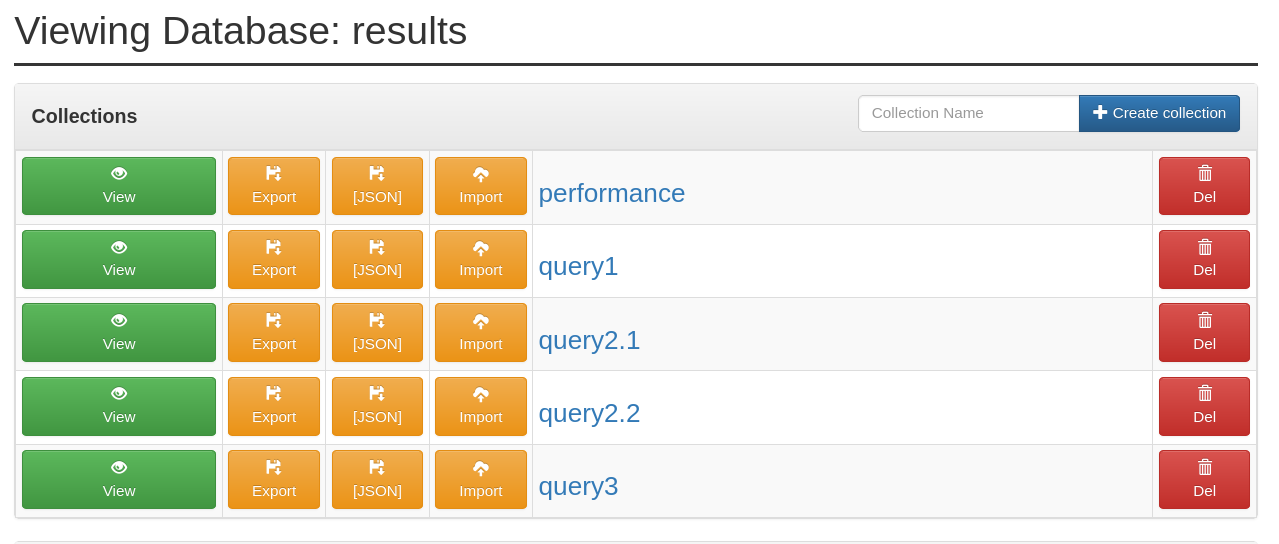
\includegraphics[width=0.5\textwidth]{res/mongo.png}}
    \caption{Schema del database MongoDB.}
    \label{fig:mongo}
\end{figure}
\subsection{Analisi delle prestazioni}
L'analisi delle prestazioni è stata effettuata per ciascuna query, in particolare sono stati valutati i tempi di esecuzione delle query a partire dai due formati di file, CSV e Parquet, e sono stati confrontati i risultati ottenuti.

\vspace{12pt}
\end{document}

    